\documentclass[]{article}
\usepackage{amsmath}
\usepackage{amssymb}
\usepackage{stmaryrd}
\usepackage{latexsym}
\usepackage{graphicx}
\usepackage{fancyhdr}
\usepackage{color}
\usepackage{listings}
\usepackage[top=1in, right=0.75in, left=0.75in]{geometry}
\usepackage[colorlinks=true, linkcolor=blue]{hyperref}

\author{
	Mohammad Hossein Shafizadegan\\
	99104781
}
\title{
	Coding Assignment 2 \\
	Machine Learning  \\
	Dr. M. Shamsollahi
}

\pagestyle{fancy}
\rhead{ML}
\lhead{CHW 2}

\newcommand{\pict}[2]{\begin{center}
		\includegraphics[width=#1\linewidth]{Fig/#2.png}
\end{center}}
\newcommand{\mat}[1]{\begin{bmatrix} #1 \end{bmatrix}}
\newcommand{\deter}[1]{\begin{vmatrix} #1 \end{vmatrix}}

\definecolor{customgreen}{rgb}{0,0.6,0}
\definecolor{customgray}{rgb}{0.5,0.5,0.5}
\definecolor{custommauve}{rgb}{0.6,0,0.8}

\definecolor{dkgreen}{rgb}{0,0.6,0}
\definecolor{gray}{rgb}{0.5,0.5,0.5}
\definecolor{mauve}{rgb}{0.58,0,0.82}

\lstset{frame=tb,
	language=python,
	aboveskip=3mm,
	belowskip=3mm,
	showstringspaces=false,
	columns=flexible,
	frame=single,	                   % adds a frame around the code
	basicstyle={\small\ttfamily},
	numbers=none,
	numberstyle=\tiny\color{gray},
	keywordstyle=\color{blue},
	commentstyle=\color{dkgreen},
	stringstyle=\color{mauve},
	breaklines=true,
	rulecolor=\color{black},
	breakatwhitespace=true,
	tabsize=3,
	numbers=left,                    % where to put the line-numbers; possible values are (none, left, right)
	numbersep=10pt,                   % how far the line-numbers are from the code
	numberstyle=\tiny\color{customgray}, % the style that is used for the line-numbers
}

\begin{document}
	\begin{figure}
		
\includegraphics[width=0.25\textwidth]{Fig/Sharif.png}
		\centering
	\end{figure}
	\maketitle
	\tableofcontents
	\newpage
		%-----------------------------------------------------------------------------------------------------------------	
	\section{Question 1}
	\subsection{Part1}
	First we load the MNIST dataset and visualize a sample of each class using the following code:
	\begin{lstlisting}
		# Step 1: Load the MNIST dataset and show an image from each class
		transform = transforms.Compose([transforms.ToTensor(), transforms.Normalize((0.5,), (0.5,))])
		train_dataset = MNIST(root='./data', train=True, download=True, transform=transform)
		test_dataset = MNIST(root='./data', train=False, download=True, transform=transform)
		
		# Show an image from each class
		classes = train_dataset.classes
		figure, axes = plt.subplots(1, len(classes), figsize=(15, 15))
		for i, ax in enumerate(axes):
			img, label = train_dataset[i]
			ax.imshow(img.squeeze().numpy(), cmap='gray')
			ax.set_title(classes[label])
			ax.axis('off')
		plt.show()
	\end{lstlisting}
	\pict{1}{F6}
	Then we define the dataloaders for the train and test set as below:
	\begin{lstlisting}
		# Step 2: Define Dataloaders for the train and test sets
		batch_size = 64
		train_loader = torch.utils.data.DataLoader(train_dataset, batch_size=batch_size, shuffle=True)
		test_loader = torch.utils.data.DataLoader(test_dataset, batch_size=batch_size, shuffle=False)
	\end{lstlisting}
	Here we define our fully connected neural network including 4 layers by completing the "FC\_Neural\_network" class. We note that for the "forward" function, there is an argument which defines the type of the activation function used for the layers.
	\begin{lstlisting}
		class FC_Neural_network(nn.Module):
			def __init__(self):
			
				super(FC_Neural_network, self).__init__()
				self.fc1 = nn.Linear(784, 256)
				self.fc2 = nn.Linear(256, 128)
				self.fc3 = nn.Linear(128, 64)
				self.fc4 = nn.Linear(64, 10)
			
			def forward(self, x, act_func):
			
				x = torch.flatten(x, 1)
				x = self.fc1(x)
				
				if act_func == "sigmoid":
				x = torch.sigmoid(x)
				elif act_func == "relu":
				x = torch.relu(x)
				elif act_func == "Leaky relu":
				x = nn.functional.leaky_relu(x, negative_slope=0.01)
				
				x = self.fc2(x)
				x = self.fc3(x)
				x = self.fc4(x)
				
				return x
	\end{lstlisting}
	In order to calculate the accuracy for the sets, we have developed the following function:
	\begin{lstlisting}
		# Accuracy calculation template
		def calculate_accuracy(network, data_loader, device, act_func, criterion):
			network.eval()
			correct = 0
			total_loss = 0.0
			with torch.no_grad():
				for inputs, labels in data_loader:
					inputs, labels = inputs.to(device), labels.to(device)
					outputs = network(inputs, act_func)
					total_loss += criterion(outputs, labels).item() * inputs.size(0)
					_, predicted = torch.max(outputs.data, 1)
					correct += (predicted == labels).sum().item()
				loss = total_loss / len(data_loader.dataset)
				accuracy = correct / len(data_loader.dataset) * 100
				return loss, accuracy
	\end{lstlisting}
	The `torch.no\_grad()` context manager is used here to optimize memory and computational efficiency during the evaluation phase of a neural network. It indicates that gradient calculations and storage are not needed because we are not training the network at this stage. By disabling gradient computation, we can save resources and make the evaluation process faster. This context manager ensures that no gradients are computed or stored during the evaluation, allowing for efficient execution of the code.\\\\
	Then we have to complete the `train()` function. It can be fully observed in the attached notebook. Then we use this function and train neural networks with different activation functions and print the results as follows:
	\begin{lstlisting}
		activation_functions = ["sigmoid", "relu", "Leaky relu"]
		
		for act_func in activation_functions:
		
			print(f"*** NN with {act_func} activation function:  ***")
			network = FC_Neural_network().to(device)
			optimizer = torch.optim.SGD(network.parameters(), lr=0.01, momentum=0.9)
			criterion = nn.CrossEntropyLoss()
			
			train(network, train_loader, test_loader, optimizer, criterion, device, act_func)
		
	\end{lstlisting}
	In the jupyter notebook, It can be seen that our networks have achieved good accuracy. 
	
	\subsection*{CIFAR10 Dataset}
	Now we train new fully connected neural network using the CIFAR10 dataset. First we have to properly load it.
	\begin{lstlisting}
		# Set random seed for reproducibility
		torch.manual_seed(42)
		
		# Data preprocessing and augmentation
		transform_train = transforms.Compose([
			transforms.RandomCrop(32, padding=4),
			transforms.RandomHorizontalFlip(),
			transforms.ToTensor(),
			transforms.Normalize((0.5, 0.5, 0.5), (0.5, 0.5, 0.5))
		])
		
		transform_val = transforms.Compose([
			transforms.ToTensor(),
			transforms.Normalize((0.5, 0.5, 0.5), (0.5, 0.5, 0.5))
		])
		
		# Load CIFAR-10 dataset
		trainset = CIFAR10(root='./data', train=True, download=True, transform=transform_train)
		train_loader = torch.utils.data.DataLoader(trainset, batch_size=64, shuffle=True)
		
		valset = CIFAR10(root='./data', train=False, download=True, transform=transform_val)
		val_loader = torch.utils.data.DataLoader(valset, batch_size=64, shuffle=False)
		
	\end{lstlisting}
	First we train the network for 20 epochs. It can be seen that the accuracy of the model after the first epoch is $39.98 \%$ which is relatively low. The point is that even after 20 epochs the performance of the model is still quite poor. The accuracy after 20 epochs is about $50 \, \%$.
	\pict{0.5}{F7}
	Now we continue training the model for 10 more epochs. Based on the figure below, There is no enhancement in the accuracy of the model even the fact that the model has experienced learning following new epochs.
	\pict{0.5}{F8}
	Indeed this section prove that the fully connected neural networks don't work well all the times and for some tasks and data, the convolutional neural networks are the solution.
	
	\newpage
	\subsection{Part 2: Transfer learning for image classification}
	Firs we load the pretrained alexnet model and the CIFAR10 dataset properly
	\begin{lstlisting}
		# Step 1: Load pre-trained AlexNet with predefined weights
		model = alexnet(pretrained=True)
		
		# Step 2: Load CIFAR10 dataset and plot an image of each class
		transform = transforms.Compose([
			transforms.Resize((224, 224)),
			transforms.ToTensor(),
		])
		
		trainset = CIFAR10(root='./data', train=True, download=True, transform=transform)
		testset = CIFAR10(root='./data', train=False, download=True, transform=transform)
	\end{lstlisting} 
	Then we visualize a sample data of each class:
	\pict{1}{F9}
	In order to reduce the training load and required time, we only use two classes of the dataset for the training process. This can be done using the following code:
	\begin{lstlisting}
		# Use only two classes, to reduce the computational load
		class_labels = [0, 4]  # Replace with the indices of the classes you want to use
		
		# Filter the dataset to include only the specified classes
		train_indices = [i for i in range(len(trainset)) if trainset.targets[i] in class_labels]
		test_indices = [i for i in range(len(testset)) if testset.targets[i] in class_labels]
		
		# Create custom datasets with only the selected classes
		filtered_train_dataset = torch.utils.data.Subset(trainset, train_indices)
		filtered_test_dataset = torch.utils.data.Subset(testset, test_indices)
		
	\end{lstlisting}
	Then using the code below, in order to fine tune the model for our classification task, we change the fully connected layer:
	\begin{lstlisting}
		# Step 4: Change fully connected layers for the classification task
		num_features = model.classifier[6].in_features
		model.classifier[6] = nn.Linear(num_features, 2)
	\end{lstlisting}
	We remember to freeze the convolutional layer using the code below:
	\begin{lstlisting}
		# Reset the weights of the fully-connected layers, but not the convolutional layers
		for param in model.features.parameters():
			param.requires_grad = False
	\end{lstlisting}
	Using a quite same process, we train the model, define the loss function and print the accuracy and results. The code can be seen vividly in the jupyter notebook.
	\pict{0.5}{F10}
	\textbf{Answer to the questions}\\
	\begin{itemize}
		\item The `.train()` function sets the model in training mode, enabling gradient computation and updating of trainable parameters.
		\item The `.eval()` function sets the model in evaluation mode, disabling gradient computation and freezing the parameters.
		\item In this example, it is important to use `.eval()` during evaluation to ensure that the model behaves consistently
		and does not update its parameters based on the evaluation data.
		\item Layers affected by `.train()` and `.eval()` functions in AlexNet:
			\begin{itemize}
				\item Dropout layers: Affected by `.train()` to apply dropout regularization during training.
				\item Batch Normalization layers: Affected by `.train()` to track running statistics and apply normalization during training.
			\end{itemize}
	\end{itemize}
	
	
		%-----------------------------------------------------------------------------------------------------------------	
	\section{Question 2}
	First we load the breast cancer dataset and visualize the data considering features one and two. Here is code developed for this section:
	\begin{lstlisting}
		# Load the Breast Cancer dataset
		data = load_breast_cancer()
		
		# Get the selected features and labels
		X = data.data[:, [feature1_index, feature2_index]]
		y = data.target
		
		# Get the class labels
		target_names = data.target_names
		
		for class_value in np.unique(y):
			# Get the indices of samples belonging to the current class
			indices = np.where(y == class_value)
			
			# Plot the samples of the current class
			plt.scatter(X[indices, 0], X[indices, 1], label=target_names[class_value])
	\end{lstlisting}
	The resulted figure can be seen below:
	\pict{0.6}{F1}
	In order to check whether and how much do these features are correlated to each other, we have calculated the correlation coefficients and the corresponding p value using the built in function "pearsonr" from scipy.stats. Here is the code:
	\begin{lstlisting}
		from scipy.stats import pearsonr
		
		# Calculate the correlation coefficient
		correlation_coef, p_value = pearsonr(X[:, 0], X[:, 1])
		
		print(f"Correlation coefficient: {correlation_coef:.4f}")
		print(f"P-value: {p_value}")
	\end{lstlisting}
	It can be seen that the correlation coefficient for features 1 and 2 are relatively small therefor, these features are not well correlated. We also note the significantly small p value which verify our result quite well. 
	\pict{0.3}{F2}
	After splitting data into train and test set using "train\_test\_split()" builtin function, we will design our decision tree model using the following code:
	\begin{lstlisting}
		from sklearn.tree import DecisionTreeClassifier
		
		# Create a decision tree classifier
		clf = DecisionTreeClassifier(criterion=splitter, max_depth=depth, random_state=42)
		
		# Fit the model on the training data
		clf.fit(X_train, y_train)
	\end{lstlisting} 
	Then using this model, we simply predict the outputs for the test data. For assessing the performance of the model, we will report the f1 score, accuracy and the corresponding confusion matrix:
	\begin{lstlisting}
		# Predict the labels for the test data
		y_pred = clf.predict(X_test)
		
		# Calculate the accuracy of the model
		accuracy = accuracy_score(y_test, y_pred)
		f1 = f1_score(y_test, y_pred)
		
		# Calculate the confusion matrix
		cm = confusion_matrix(y_test, y_pred)
	\end{lstlisting}
	Finally in a loop, we use this code for different tree depth, then we print and visualize the results as well.
	\begin{lstlisting}
		splitter = 'entropy'
		depths = [2, 5, 10]
		
		# Fit and evaluate the decision tree for each depth
		for depth in depths:
			# Create a decision tree classifier
			clf = DecisionTreeClassifier(criterion=splitter, max_depth=depth, random_state=42)
			
	\end{lstlisting}
	The results can be seen below:
	\begin{center}
		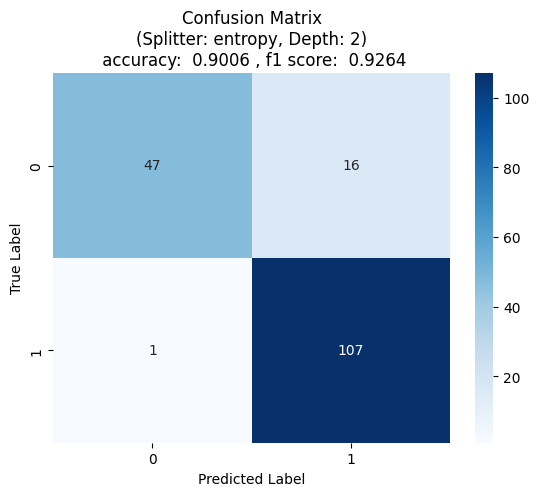
\includegraphics[width=0.3\linewidth]{Fig/F3.png}
		\qquad
		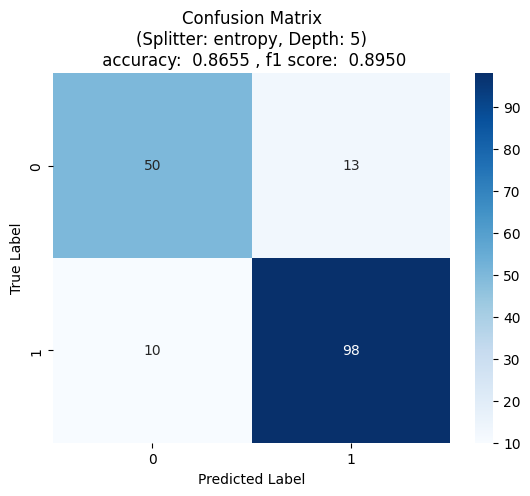
\includegraphics[width=0.3\linewidth]{Fig/F4.png}
		\qquad
		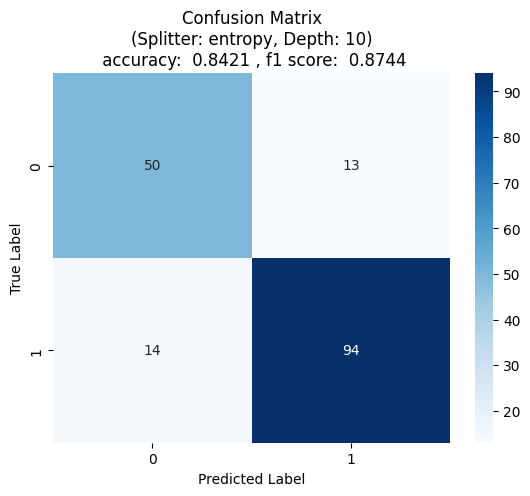
\includegraphics[width=0.3\linewidth]{Fig/F5.png}
	\end{center}
	It can be seen that as we increase the depth of the tree the accuracy will decrease regarding the concept of overfitting.\\\\
	The accuracy for other algorithms we used before is a bit higher as KNN and SVM classifiers achieved accuracy of 96.5 \% but the best accuracy for decision tree is 90 \%. We should note that we have to assess other measures like f1 score or sensitivity too.
\end{document}